
\begin{figure}[h!]
\centering
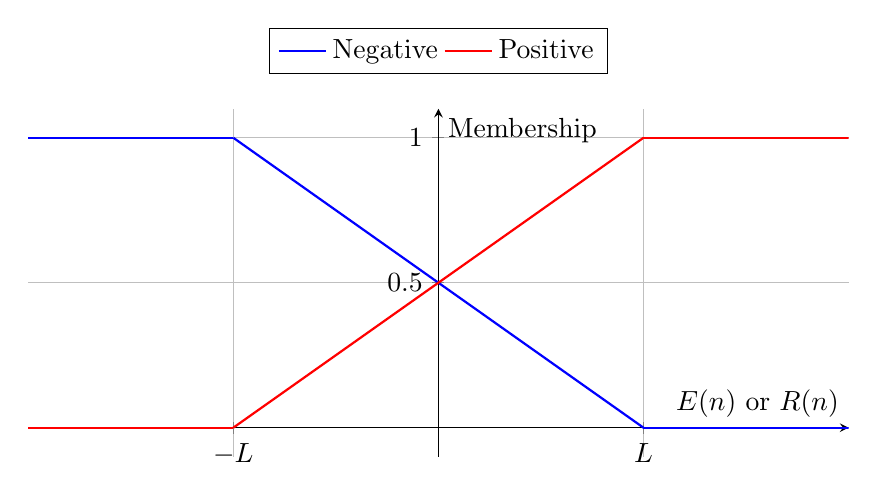
\begin{tikzpicture}
\begin{axis}[
    axis lines=middle,
    xlabel={$E(n)$ or $R(n)$},
    ylabel={Membership},
    ymin=-0.1, ymax=1.1,
    xmin=-20, xmax=20,
    xtick={-10, 0, 10},
    xticklabels={$-L$, $0$, $L$},
    ytick={0, 0.5, 1},
    grid=both,
    width=12cm, height=6cm,
    legend style={at={(0.5,1.1)}, anchor=south, legend columns=-1}
]

% -------- Negative MF (blue) --------
\addplot[domain=-20:-10, thick, blue, samples=2, forget plot] {1};
\addplot[domain=-10:10, thick, blue, samples=100] {(-x + 10)/20};
\addlegendentry{Negative}
\addplot[domain=10:20, thick, blue, samples=2, forget plot] {0};

% -------- Positive MF (red) --------
\addplot[domain=-20:-10, thick, red, samples=2, forget plot] {0};
\addplot[domain=-10:10, thick, red, samples=100] {(x + 10)/20};
\addlegendentry{Positive}
\addplot[domain=10:20, thick, red, samples=2, forget plot] {1};

\end{axis}
\end{tikzpicture}
\caption{Input fuzzy sets: Negative and Positive}
\label{fig:fig1}
\end{figure}